\PassOptionsToPackage{force}{filehook}
%https://tex.stackexchange.com/questions/462793/latex-error-option-clash-for-package-geometry

%para armar un preambulo
\documentclass{beamer}


\usepackage[utf8]{inputenc}
\usepackage{amsmath}
\usepackage{amssymb}% http://ctan.org/pkg/amssymb
\usepackage{amsfonts}
\usepackage{pifont}% http://ctan.org/pkg/pifont
%https://tex.stackexchange.com/questions/42619/x-mark-to-match-checkmark
\newcommand{\cmark}{\ding{51}}
\newcommand{\xmark}{\ding{55}}
%\usepackage{amsfonts}
\usepackage{graphicx} 
\usepackage{subcaption}
\usepackage{hyperref}
\usepackage{cancel}
\usepackage{wrapfig}
\usepackage{enumitem}
\usepackage{comment}
\hypersetup{
	colorlinks=true,
	linkcolor=blue,
	filecolor=magenta,      
	urlcolor=cyan,
}
\newtheorem*{proposicion}{Proposici\'on}
\newtheorem*{teorema}{Teorema}
\renewcommand*{\proofname}{Demostraci\'on}
\newtheorem*{ejercicio}{Ejercicio}
\usepackage{pgf,tikz}
\usetikzlibrary{positioning}
\usetikzlibrary{arrows,patterns}
\usetikzlibrary{arrows.meta}
\usepackage[spanish, activeacute]{babel} %Definir idioma español
\usepackage[utf8]{inputenc} %Codificacion utf-8
\usepackage{multirow}

%   Esconder las soluciones
\newif\ifhideproofs
\hideproofstrue %uncomment to hide proofs

\ifhideproofs
\usepackage{environ}
\NewEnviron{hide}{}
\let\solucion\hide
\let\endsolucion\endhide
\fi

\usepackage{color}
\usepackage{mathpazo}
\usepackage{hyperref}
\usepackage{multimedia}
\usepackage{graphicx}
\usepackage{textcomp}
\usepackage[spanish, activeacute]{babel} 
\usepackage{graphicx} 
\usepackage{booktabs}
\usepackage{cite}
\usepackage{hyperref}
\usepackage{multicol}
\usepackage{multirow,array}

\usepackage{mathrsfs}
%\usepackage{amssymb}

\usepackage{tabularx}
    \newcolumntype{L}{>{\raggedright\arraybackslash}X}
        %\newcolumntype{b}{>{\hsize=1.5\hsize}X}
    %\newcolumntype{s}{>{\hsize=.9\hsize}X}

\usepackage{amsthm}
\newtheorem{thm}{Teorema}
\newtheorem{lem}[thm]{Lema}
\newtheorem{axiom}[thm]{Axioma}
\newtheorem{prop}[thm]{Proposici\'on}
\newtheorem{coro}[thm]{Corolario}
\theoremstyle{definition}
\newtheorem{defn}{Definici\'on}
\DeclareGraphicsExtensions{.pdf,.jpeg,.png,.eps}
\usetheme{CambridgeUS}
\setbeamertemplate{navigation symbols}{}

%Paréntisis y otros
\newcommand{\cmc}{\overset{m.c.}{\rightarrow}}
\newcommand{\p}[1]{\left(#1\right)}
\newcommand{\cor}[1]{\left[#1\right]}
\newcommand{\lla}[1]{\left\{#1\right\}}
\newcommand{\eps}{\varepsilon}
\newcommand{\lol}{\mathcal{L}}
\newcommand{\RR}{\mathbb{R}}
\newcommand{\QQ}{\mathbb{Q}}
\newcommand{\NN}{\mathbb{N}}
\newcommand{\paren}[1]{\left(#1\right)}
\newcommand{\corc}[1]{\left[#1\right]}
\newcommand{\llav}[1]{\left\lbrace#1\right\rbrace}
\newcommand{\partt}[1]{\left(\text{#1}\right)}
\newcommand{\corctt}[1]{\left[\text{#1}\right]}
\newcommand{\llavtt}[1]{\left\lbrace\text{#1}\right\rbrace}
\makeatletter
\def\munderbar#1{\underline{\sbox\tw@{$#1$}\dp\tw@\z@\box\tw@}}
\makeatother

%\usepackage[scr=rsfs,cal=boondox]{mathalfa}
\usepackage[scr=esstix,cal=boondox]{mathalfa}

% \usepackage{mdframed}
% \newmdtheoremenv{solucion}{Soluci\'on}

% Enmarcar las soluciones
% \newenvironment{solu}
% {%
% \begin{framed}
%   \begin{solucion}
%   }%
%     {%     
%   \end{solucion}
% \end{framed}
% }

%   Esconder las soluciones
\newif\ifhideproofs
%\hideproofstrue %uncomment to hide proofs

\ifhideproofs
\usepackage{environ}
\NewEnviron{hide}{}
\let\solucion\hide
\let\endsolucion\endhide
\fi

\decimalpoint

%Graficos y cosas
\usepackage{amssymb}
\usepackage{tikz}
\usepackage{pgfplots}
\usepackage{mathtools}
\usepackage{xcolor}
%\pgfplotsset{compat=1.9}
\usepgfplotslibrary{fillbetween,decorations.softclip}
\pgfplotsset{compat = newest}
\usepackage{pst-func}
\usepackage{pstricks}
\usepackage{pst-plot}

% Comando para usar multiples footnotes en un align environment

\makeatletter
\newcommand{\AlignFootnote}[1]{%
    \ifmeasuring@
    \else
        \footnote{#1}%
    \fi
}
\makeatother

%https://tex.stackexchange.com/questions/82782/footnote-in-align-environment


\DeclareGraphicsExtensions{.pdf,.jpeg,.png,.eps}
\usepackage{tikz}
%\usepackage{tikz-cd}
\usetikzlibrary{decorations}
%\usetikzlibrary{snakes}
\usetikzlibrary{cd}

\useoutertheme{split}
\useinnertheme{rounded}


%\beamertemplatenavigationsymbolsempty  %removes navigation bar
\definecolor{rosee}{rgb}{0.7,0.05,0.25}
\definecolor{pacificorange}{cmyk}{0,.6,1,0} %approved Pacific colors 2010
\definecolor{pacificgray}{cmyk}{0,.15,.35,.60}
\definecolor{pacificlgray}{cmyk}{0,0,.2,.4}
\definecolor{pacificcream}{cmyk}{.05,.05,.15,0}
\definecolor{deepyellow}{cmyk}{0,.17,.80,0}
\definecolor{lightblue}{cmyk}{.49,.01,0,0}
\definecolor{lightbrown}{cmyk}{.09,.15,.34,0}
\definecolor{deepviolet}{cmyk}{.79,1,0,.15}
\definecolor{deeporange}{cmyk}{0,.59,1,18}
\definecolor{dustyred}{cmyk}{0,.7,.45,.4}
\definecolor{grassgreen}{RGB}{92,135,39}
\definecolor{pacificblue}{RGB}{59,110,143}
\definecolor{pacificgreen}{cmyk}{.15,0,.45,.30}
\definecolor{deepblue}{cmyk}{1,.57,0,2}
\definecolor{turquoise}{cmyk}{.43,0,.24,0}
\definecolor{gren}{rgb}{0.2,0.8,0.5}
\definecolor{orang}{rgb}{1,0.64,0}
\definecolor{amethyst}{rgb}{0.6, 0.4, 0.8}
\definecolor{dodgerblue}{rgb}{0.12, 0.56, 1.0}
\definecolor{fandango}{rgb}{0.71, 0.2, 0.54}
\definecolor{forestgreen(traditional)}{rgb}{0.0, 0.27, 0.13}
\definecolor{iris}{rgb}{0.35, 0.31, 0.81}
\definecolor{jazzberryjam}{rgb}{0.65, 0.04, 0.37}
\definecolor{mediumjunglegreen}{rgb}{0.11, 0.21, 0.18}
\definecolor{mediumpersianblue}{rgb}{0.0, 0.4, 0.65}
\definecolor{midnightgreen}{rgb}{0.0, 0.29, 0.33}
\definecolor{orangee}{rgb}{1.0, 0.5, 0.0}

% There are many different themes available for Beamer. A comprehensive
% list with examples is given here:
% http://deic.uab.es/~iblanes/beamer_gallery/index_by_theme.html
% You can uncomment the themes below if you would like to use a different
% one:
%\usetheme{AnnArbor} %boca
%\usetheme{Antibes} %azul y gris
%\usetheme{Bergen} %barra who where
%\usetheme{Berkeley} %bordes
%usetheme{Berlin} %blanco y azul
%\usetheme{Boadilla}
%\usetheme{boxes}
\usetheme{CambridgeUS}
%\usetheme{Copenhagen}
%\usetheme{Darmstadt}
%\usetheme{default}
%\usetheme{Frankfurt}
%\usetheme{Goettingen}
%\usetheme{Hannover}
%\usetheme{Luebeck}
%\usetheme{Malmoe}
%\usetheme{Marburg}
%\usetheme{Montpellier}
%\usetheme{PaloAlto}
%\usetheme{Pittsburgh}
%\usetheme{Rochester}
%\usetheme{Singapore}
%\usetheme{Szeged}
%\usetheme{Warsaw}

%\usecolortheme{beaver}
%\usecolortheme{whale}
%\usecolortheme{orchid}
%\usecolortheme{wolverine}
%\usecolortheme[named=pacificblue]{structure} %replaces the blue of Copenhagen with Pacific orange

\definecolor{myNewColorA}{rgb}{0,0,100}
\definecolor{myNewColorB}{rgb}{0,100,100}
\definecolor{myNewColorC}{rgb}{0,200,100}
\definecolor{myNewColorD}{rgb}{0,100,200}

%\setbeamercolor*{palette primary}{bg=myNewColorA, fg = black}
%\setbeamercolor*{palette secondary}{bg=myNewColorB, fg = black}
%\setbeamercolor*{palette tertiary}{bg=myNewColorC, fg = black}
%\setbeamercolor*{palette quaternary}{bg=myNewColorD, fg = black}

\setbeamercolor*{palette primary}{bg=rosee, fg = white}
\setbeamercolor*{palette secondary}{bg=gren, fg = white}
\setbeamercolor*{palette tertiary}{bg=-red!75!, fg = white}
\setbeamercolor*{palette quaternary}{bg=-red!75!, fg = white}

\newtheorem{proposition}{Proposici\'on}
\newcommand{\ton}{\underset{n\to\infty}{\longrightarrow}}
\newcommand{\cp}{\overset{P}{\rightarrow}}
\newcommand{\cw}{\overset{d}{\rightarrow}}

%\expandafter\def\expandafter\insertshorttitle\expandafter{%
 % \insertshorttitle\hfill%
  %\insertframenumber\,/\,\inserttotalframenumber}

%\mode
%<all>

%Para agrandar el espacio entre renglones de las tablas
%https://tex.stackexchange.com/questions/26690/how-to-add-extra-spaces-between-rows-in-tabular-environment
\renewcommand{\arraystretch}{1.5}

\usepackage{color, xcolor}
\definecolor{codegreen}{rgb}{0,0.6,0}
\definecolor{codegray}{rgb}{0.5,0.5,0.5}
\definecolor{codepurple}{rgb}{0.58,0,0.82}
\definecolor{backcolour}{rgb}{0.95,0.95,0.92}

\usepackage{listings}
\lstdefinestyle{mystyle}{
  backgroundcolor=\color{backcolour},   
  commentstyle=\color{codegreen},
  language = R,
  % commentchar=\#,
  keywordstyle=\color{magenta},
  numberstyle=\tiny\color{codegray},
  stringstyle=\color{codepurple},
  basicstyle=\ttfamily\footnotesize,
  breakatwhitespace=false,         
  breaklines=false,                 
  captionpos=b,                    
  frame=single,
  keepspaces=false,
  % numbers=left,                    
  % numbersep=pt,                  
  % columns=flexible,
  stepnumber=1,
  resetmargins=true,
  showspaces=false,                
  showstringspaces=false,
  showtabs=false,                  
  tabsize=1
}
\lstset{style=mystyle}
  
\def\mydate{\leavevmode\hbox{\twodigits\day/\twodigits\month/\the\year}}
\def\twodigits#1{\ifnum#1<10 0\fi\the#1}

\usepackage[final]{pdfpages}

% PARA AGREGAR IMAGEN EN EL FONDO DE LAS SLIDES
\usebackgroundtemplate%
%{%
 %
\includegraphics[width=\paperwidth,height=\pape%rheight]{slides1/fondo.png}%  
%}

\newtheorem*{remark}{Observaci\'on}
\DeclareMathOperator*{\argmax}{arg\,max}
\DeclareMathOperator*{\argmin}{arg\,min}

\begin{document}

\title{\color{rosee}An\'alisis Estad\'istico}
\subtitle{\color{rosee}Test de hip\'otesis 1\footnote{Basado en las notas de Ezequiel Smucler}}

\institute{UTDT}
\date{\today}

\begin{frame}
  \maketitle
\end{frame}

\begin{frame}{\color{rosee}Test de hip\'otesis (motivación)} \small
  \begin{block}{Introducci\'on}
    Un par\'ametro puede ser estimado a partir de una muestra por
    \begin{itemize}
    \item un solo n\'umero (\textbf{estimaci\'on puntual});
    \item un intervalo de valores posibles (\textbf{intervalo de confianza}).
    \end{itemize}
    Frecuentemente \textbf{el objetivo} de una investigaci\'on \textbf{no s\'olo es estimar} el
    valor del par\'ametro \textbf{sino decidir cu\'al} -\textbf{entre dos afirmaciones} sobre el par\'ametro- mutuamente excluyentes- \textbf{es verdadera}.
  \end{block}
\textbf{Ejemplos:}
    \begin{itemize}[leftmargin=*]
    \item ¿La mayoría de la población argentina está a favor de la ley de etiquetado?\medskip % (es $p > 0.5$?)  
    \item ¿Disminuye significativamente la cantidad de horas trabajadas cuando se hace \textit{home-office}? %¿Existe discriminación entre los salarios de hombres y mujeres?\medskip% (es $\mu_H - \mu_M \neq 0$?)\medskip 
    %\item Introducimos las ideas mediante un ejemplo concreto...
\end{itemize}
   
\end{frame}

\begin{frame}{\color{rosee} Tests de hipótesis}\small
\textbf{Tests exactos}
\begin{center}
\begin{tabular}{|c|c|c|c|}
\hline
 Test para   &  Datos & Estadístico $t(\munderbar{X})$& Distr. bajo $H_0$\\
 \hline
 $\mu$    & $X_i\stackrel{iid}{\sim}N(\mu,\sigma^2)$  & $\frac{\sqrt{n}(\overline{X}_n-\mu)}{\sigma}$ & $\frac{\sqrt{n}(\overline{X}_n-\mu_0)}{\sigma}\sim N(0,1)$\\
 \hline
  $\mu$    & $X_i\stackrel{iid}{\sim}N(\mu,\sigma^2)$  & $\frac{\sqrt{n}(\overline{X}_n-\mu)}{S}$ & $\frac{\sqrt{n}(\overline{X}_n-\mu_0)}{\sigma}\sim t_{n-1}$\\
 \hline
  $\sigma^2$    & $X_i\stackrel{iid}{\sim}N(\mu,\sigma^2)$  & $\frac{(n-1)S^2}{\sigma^2}$ & $\frac{(n-1)S^2}{\sigma_0^2}\sim \chi^2_{n-1}$\\
 \hline
\end{tabular}
\end{center}

\textbf{Tests asintóticos}

\begin{center}
\begin{tabular}{|c|c|c|c|}
\hline
 Test para   &  Datos & Estadístico $t(\munderbar{X})$.& Distr. bajo $H_0$\\
 \hline
 $\mu$    & $X_i\stackrel{iid}{\sim}$  & $\frac{\sqrt{n}(\overline{X}_n-\mu)}{S}$ & $\frac{\sqrt{n}(\overline{X}_n-\mu_0)}{S}\stackrel{D}{\to} N(0,1)$\\
 \hline
  $p$    & $X_i\stackrel{iid}{\sim}Be(p)$  & $\frac{\sqrt{n}(\overline{X}_n-p)}{\overline{X}_n(1-\overline{X}_n)}$ & $\frac{\sqrt{n}(\overline{X}_n-p_0)}{\overline{X}_n(1-\overline{X}_n)}\stackrel{D}{\to}N(0,1)$\\
  \hline
   $\theta$\footnotemark    & $X_i\stackrel{iid}{\sim}$  & $\frac{\sqrt{n}(\widehat{\theta}_n-\theta)}{\widehat{V(\theta)}}$ & $\frac{\sqrt{n}(\widehat{\theta}_n-\theta_0)}{\widehat{V(\theta)}}\stackrel{D}{\to} N(0,1)$\\
 \hline
\end{tabular}
\end{center}

\footnotetext{Este test se conoce como \textbf{test de Wald} para $\theta$. $\widehat{\theta}_n$ es un estimador \textbf{asintóticamente normal} de $\theta$. En el caso particular que el estimador sea $\widehat{\theta}_{MV}$, vale que $V(\theta)=I_{1}^{-1}(\theta)$ y $\widehat{V(\theta)}=V(\widehat{\theta})$ es un estimador consistente de $V(\theta)$.}
    
\end{frame}

\begin{frame}{\color{rosee}Elementos de un test de hipótesis}\small
Para realizar un test de hipótesis vamos a hacer un \textbf{contraste} entre las hipótesis que tenemos y los datos que recolectamos. Para conducir un test de hipótesis tenemos que definir varios conceptos.

\begin{columns}
    \begin{column}[t]{0.48\textwidth}
    \textbf{Hipótesis:}
        \begin{itemize}
            \item Hipótesis nula $H_0$ e hipótesis alternativa $H_1$.
            \item estadístico $t(\munderbar{X})$ y distribución bajo $H_0$.
            \item Probabilidad de error de tipo I, $\alpha$ (nivel de significatividad/del test).
            \item Probabilidad de error de tipo II, $\beta$. 
            \item Valor crítico $t_c$.
            \item Regla de decisión para rechazar $H_0$, $\mathcal{R}$.
        \end{itemize}
    \end{column}
    \begin{column}[t]{0.48\textwidth}
    \textbf{Contraste empírico:}
          \begin{itemize}
            \item Datos observados $\munderbar{x}$.
            \item Estadístico observado $t_{\text{obs}}$.
            \item $p$-valor.
        \end{itemize}

        \vspace{20pt}

        \textbf{Comentario importante:} A partir del planteo de $H_0$ y $H_1$, si se elige $\alpha$ quedan automáticamente determinados $\mathcal{R}$ y $\beta$. Similarmente, si se elige $\mathcal{R}$ quedan determinados $\beta$ y $\alpha$.
    \end{column}
\end{columns}
\end{frame}


\begin{frame}{\color{rosee}Tipos de hipótesis y test}\small
  \textbf{Tipos de hip\'otesis}\small
    \begin{itemize}
    \item Hip\'otesis nula \textbf{simple}: $\theta = \theta_0$.
    \item Hip\'otesis nula \textbf{compuesta}: $\theta \leq \theta_0$, \quad 
      $\theta \geq \theta_0$.
    \end{itemize}

    Bajo una hipótesis nula es \textbf{simple} hay un único valor verdadero del parámetro $\theta$, $\theta_0$. Bajo una hipótesis nula \textbf{compuesta} hay muchos único valor verdadero del parámetro $\theta$. No obstante, si $H_0$ es compuesta tomaremos el valor $\theta_0$ para construir el estadístico bajo $H_0$. Explicaremos luego por qué.
    
  \vspace{5pt}
  
\textbf{Tipos de test (bilateral y unilateral a una cola) con $H_0$ simple.}
  \begin{columns}
        \begin{column}{0.32\textwidth}
        \begin{center}
          \textbf{Test a cola derecha}
          \begin{itemize}
          \item $H_0$:  $\theta = \theta_0$
          \item $H_1$: $\theta > \theta_0$
          \end{itemize}
          \end{center}
      \end{column}
        \begin{column}{0.32\textwidth}
        \begin{center}
        \textbf{Test a cola izquierda}
           \begin{itemize}
          \item $H_0$: $\theta = \theta_0$
          \item$H_1$: $\theta < \theta_0$
          \end{itemize}
          \end{center}
      \end{column}
        \begin{column}{0.32\textwidth}
        \begin{center}
        \textbf{Test bilateral}
           \begin{itemize}
          \item $H_0$: $\theta = \theta_0$
          \item$H_1$: $\theta \neq \theta_0$
          \end{itemize}
          \end{center}
      \end{column}
  \end{columns}

\vspace{8pt}

  El tipo de test determinará cómo se determina $\mathcal{R}$ una vez determinado $\alpha$ y también el $p$-valor. (Discusión sobre \href{https://stats.stackexchange.com/questions/23142/when-to-use-fisher-and-neyman-pearson-framework}{\textbf{Fisher} vs. \textbf{Neyman-Pearson}}).
\end{frame}

\begin{frame}{\color{rosee} Test de hipótesis primer ejemplo}\small

    Las \textbf{hip\'otesis estad\'isticas} son afirmaciones sobre el valor de un par\'ametro desconocido en la población.
Supongamos que queremos determinar si con \textit{home-office} se trabaja menos; esto equivale a decidir entre dos posibles \textbf{hip\'otesis} mutuamente excluyentes:
    \begin{description} 
    \item[Hip\'otesis nula] $H_0$: Con \textit{home-office} se trabaja la misma cantidad de hs.
    \item[Hip\'otesis alternativa] $H_1$: Con \textit{home-office} se trabaja menos hs.
    \end{description} 

   Consideramos el estadístico
    aleatoria
     \[t(\munderbar{X})=\frac{\sqrt{n}(\overline{X}_n-\mu)}{\sigma}\]
     
      \noindent donde $X_i\stackrel{iid}{\sim}N(\mu,\sigma^2)$ mide la cantidad de horas trabajadas el día $i-$\'esimo y $\sigma=2$.
   

\end{frame}


\begin{frame}{\color{rosee}Sobre el planteo de las hipótesis} \small

  ¿Por qué definimos $H_0$ y $H_1$ de esta manera?
  
En general, la hipótesis nula $H_0$ codifica el \href{https://www.youtube.com/watch?v=yE07FbWmew8&ab_channel=DisneyMusicVEVO}{`status quo'}:\medskip
\begin{enumerate}
\item La moneda que estamos testeando es una moneda balanceada.
\item La droga que estamos probando no tiene efecto sobre la presión arterial.
\item La política pública que se implementó no tuvo efecto sobre la tasa de desempleo.
\item El nuevo proceso de producción no mejora la productividad.
\end{enumerate}
En estos casos, la hipótesis alternativa $H_1$ codifica un `descubrimiento'. Informalmente, que encontramos algo nuevo que no sabíamos antes.
  
  \medskip
Por esta razón la carga de la prueba cae sobre la hipótesis alternativa $H_1$.... 

\end{frame}


\begin{frame}{\color{rosee}Sobre el planteo de las hipótesis} \small
La razón por la que hacemos esto queda claro con el siguiente ejemplo citando el art\'iculo 11 de la Declaraci\'on Universal de los Derechos Humanos

``Toda persona acusada de delito tiene derecho a que se presuma su
     inocencia mientras no se pruebe su culpabilidad [\dots]''

  El esp\'iritu de la metodolog\'ia es an\'alogo al de un juicio
  legal. En este caso las hip\'otesis nula y alternativa son:
  \begin{center}
   $H_0$: el acusado es inocente vs $H_1$: el acusado es culpable
  \end{center}
   La acusaci\'on proviene de una sospecha de culpabilidad. La hip\'otesis $H_0$ se establece en oposici\'on a $H_1$ y se mantiene a menos que la evidencia apoye a $H_1$.
  Por defecto, la hip\'otesis \textit{el acusado es inocente} es
  cierta. La hip\'otesis nula ser\'a rechazada en favor de la
  hip\'otesis alternativa el \textit{acusado es culpable} si hay
  suficiente evidencia.
  \begin{itemize}
  \item \textbf{Se rechaza $H_0$} cuando el jurado encuentra evidencia suficiente para afirmar que el acusado es culpable.
  \item Si \textbf{no se rechaza $H_0$}, esto no implica que el acusado sea
    inocente sino que la evidencia fue insuficiente para lograr una condena. El jurado no necesariamente acepta $H_0$ sino que
      no rechaza $H_0$.
  \end{itemize}
\end{frame}

\begin{frame}{\color{rosee}Sobre el rechazo (o no) de $H_0$} 
Diremos que:\medskip
  
\begin{itemize}
    \item Rechazaremos la hip\'otesis nula en favor de la alternativa cuando
    observemos una muestra que es dif\'icil de esperar si la hip\'otesis
    nula fuera cierta.\medskip

    

    \item En cambio, cuando no tenemos suficiente evidencia como para rechazar $H_0$, \textbf{no decimos que aceptamos }$H_0$; en cambio decimos que \textit{no hay suficiente evidencia como para poder rechazar $H_0$} (ver \href{https://es.wikipedia.org/wiki/Falsacionismo}{Falsacionismo popperiano}).\footnote{Como veremos más adelante, al no rechazar $H_0$ podríamos estar cometiendo el error de tipo II, y el método de testeo no nos permite controlar la probabilidad de cometer este error. Por este motivo es preciso que seamos cautos respecto de la veracidad de $H_0$ cuando no la podemos rechazar.}
\end{itemize}
  
\end{frame}



\begin{frame}{\color{rosee}Elementos del test}\small

Partiendo de hipótesis, $H_0: \mu=40$ vs $H_1: \mu<40$

Además de las hipótesis, necesitamos dos elementos más para el planteo del test
    \begin{enumerate}
    \item Un \textbf{estad\'istico de contraste} (o estadístico del test): 
    \begin{itemize}
        \item En el ejemplo, el estadístico de contraste es $t(\munderbar{X}) =\frac{\sqrt{n}(\overline{X}_n-\mu)}{2}\sim N(0,1)$. Bajo $H_0$, vale que $t_0(\munderbar{X}) =\frac{\sqrt{n}(\overline{X}_n-40)}{2}\sim N(0,1)$.\medskip
    
    \end{itemize}
    \item Una \textbf{regi\'on de rechazo} ($\mathcal{R}$) es un conjunto de valores que toma estad\'istico (bajo $H_0$) donde los cuales decidimos rechazar $H_0$.
        \begin{itemize}
        \item Si el gerente quiere tomar la decisión de mantener o quitar el \textit{home-office} podría elegir que si los trabajadores trabajan menos de $39$hs semanales 
 $\mathcal{R} = \left\{t_0(\munderbar{X}) \geq \frac{\sqrt{n}(39-40)}{2}\right\}$.\medskip
        \item Luego discutiremos c\'omo elegir $\mathcal{R}$ en cada caso.
        \item Es importante notar que la elección de $\mathcal{R}$ es arbitraria y determinará el valor de $\alpha$.
    \end{itemize}
    \end{enumerate}

\end{frame}


\begin{frame}{\color{rosee}Tipos de error}\small
  
    Podr\'iamos incurrir en dos tipos de error:
    \begin{itemize}
    \item Rechazar $H_0$ cuando es ``verdadera'' (si el verdadero $\theta\in H_0$).
    \item no rechazar $H_0$ cuando es ``falsa'' (si el verdadero $\theta\not\in H_0$).
    \end{itemize}
    
    \begin{table}
      \begin{tabular}{|rcc|}
        \hline
        & Rechazamos $H_0$  & no rechazamos $H_0$ \\
        \hline
        Bajo $H_0$ & {\bf error tipo I} & no hay error         \\
        Bajo $H_1$  & no hay error       & {\bf  error tipo II} \\
        \hline
      \end{tabular}
    \end{table}
    luego analizaremos las probabilidades de cometer estos errores (que \textbf{dependerán de como elijamos la zona de rechazo $\mathcal{R}$}).
  
 \end{frame}


\begin{frame}{\color{rosee}Probabilidades de cometer errores}\small
    \begin{table}
      \begin{tabular}{|rcc|}
      \hline
        & Rechazamos $H_0$  & no rechazamos $H_0$ \\
      \hline
        $H_0$ es cierta   &  $\boldsymbol{\alpha} = P(t_0(\munderbar{X})\in\mathcal{R}|H_0 \text{ cierta})$   &  -  \\
        $H_0$ es falsa    & -  & $\boldsymbol{\beta}= P(t_0(\munderbar{X})\notin\mathcal{R}|H_0 \text{ falsa})$ \\
        \hline
      \end{tabular}
    \end{table}
    \medskip
\begin{itemize}
    \item En muchas aplicaciones \textbf{se considera más grave cometer un error de tipo I que un error de tipo II}. Este es el caso, por ejemplo, cuando la hipótesis nula dice que el acusado es inocente. Un error de tipo I en este caso es decirle a un inocente que tiene que ir a prisión.\medskip
    \item \color{blue}{Elegimos $\mathcal{R}$ para garantizar que la probabilidad de cometer el error tipo I (el más grave) sea como mucho $\alpha$}.\color{black}
\item  \color{red}{Importante}: $\alpha \neq 1- \beta$! \color{black} 
\end{itemize}
\end{frame}

\begin{frame}[fragile]{\color{rosee}$H_0:\mu = \mu_0$ vs $H_1: \mu< \mu_0$ ($\alpha$ vs $\beta$)}

\pgfmathdeclarefunction{gauss}{3}{%
  \pgfmathparse{1/(#3*sqrt(2*pi))*exp(-((#1-#2)^2)/(2*#3^2))}%
}
\begin{center}

    \begin{tikzpicture}
\begin{axis}[
  no markers, 
  domain=-3:3, 
  samples=100,
  ymin=0,
  axis lines*=left, 
  xlabel=$\overline{x}_n$,
  every axis y label/.style={at=(current axis.above origin),anchor=south},
  every axis x label/.style={at=(current axis.right of origin),anchor=west},
  height=5cm, 
  width=12cm,
  xtick=\empty, 
  ytick=\empty,
  enlargelimits=false, 
  clip=false, 
  axis on top,
  grid = major,
  hide y axis
  ]

 \addplot [very thick,cyan!50!black] {gauss(x, -0.7, 0.7)};
 \addplot [fill=cyan!50!, draw=none, domain=-0.5:3] {gauss(x,-0.7,0.7)} \closedcycle;
 \addplot [very thick,red!50!black] {gauss(x, 0.7, 0.7)};
 \addplot [fill=red!50, draw=none, domain=-3:-0.5] {gauss(x,0.7,0.7)} \closedcycle;

\pgfmathsetmacro\valueA{gauss(0.7,0.7,0.7)}
\pgfmathsetmacro\valueB{gauss(-0.7,-0.7,0.7)}
\pgfmathsetmacro\valueC{gauss(-0.5,-0.7,0.7)}

\draw [thick, gray, dotted]  (axis cs:0.7,0) -- (axis cs:0.7,\valueA);
\draw [thick, gray, dotted]  (axis cs:-0.7,0) -- (axis cs:-0.7,\valueB);
\draw [thick, gray]  (axis cs:-0.5,0) -- (axis cs:-0.5,\valueC);

\node[] at (axis cs:-0.6,0.08) {$\alpha$};
\node[] at (axis cs:0,0.08) {$\beta$};
\node[] at (axis cs:-1,0.3) {$1-\beta$};
\node[] at (axis cs:0.7,0.3) {$1-\alpha$};

%\draw [yshift=1cm, latex-latex](axis cs:2, 0) -- node [fill=white] {$\beta^{'}= 0.0011$} (axis cs:4, 0);
%\draw [yshift=1cm, latex-latex](axis cs:-4, 0) -- node [fill=white] {$1-\beta^{'}= 0.9989$} (axis cs:2, 0);

\draw [yshift=1cm, latex-latex](axis cs:-3, -0.3) -- node [fill=white] {$\mathcal{R}$} (axis cs:-0.5, -0.3);
\draw [yshift=1cm, latex-latex](axis cs:-0.5, -0.3) -- node [fill=white] {$\mathcal{R}^C$} (axis cs:3, -0.3);

\node[above] at (axis cs:-1, 0.6) {\color{cyan!50!black}Bajo $H_1$};
\node[above] at (axis cs:1, 0.6) {\color{red!50!black}Bajo $H_0$};

%\node[below] at (axis cs:1.47, 0)  {$z_{0.9251}=-1.44$}; 
\node[below] at (axis cs:-0.7, 0)  {$\mu$}; 
\node[below] at (axis cs:0.7, 0)  {$\mu_0$};  
\node[below] at (axis cs: -0.5, 0)  {$\bar{x}_c$};
\end{axis}
\end{tikzpicture} 
\end{center}
    \begin{itemize}
    \item Con $n$ fijo, elegir un valor crítico $\bar{x}_c$ para $\mathcal{R}$ con tal disminuir $\alpha$ resulta en un mayor valor de
      $\beta$ para cualquier valor del par\'ametro bajo la hipótesis alternativa.
    \end{itemize}
\end{frame}

\begin{frame}{\color{rosee}Probabilidad de error de tipo II, $\beta$}\small
  
    En general la probabilidad de error de tipo II, $\beta=\beta(\mu)$, depende del valor de $\mu$ que consideremos. 
    \begin{align*}
      \beta(\mu)
      &= P_{\mu}\left(t_0(\munderbar{X}) \geq \frac{\sqrt{n}(39-40)}{2}\right) = P\left(Z \geq \frac{\sqrt{n}(39-40)}{2}\color{rosee}+\frac{\sqrt{n}(40-\mu)}{2}\color{black}\right)
    \end{align*}

\textbf{Importante:} Cuando escribimos $P_{\mu}$ estamos diciendo que la distribución de $t(\munderbar{X})=\frac{\sqrt{n}(\overline{X}_n-\mu)}{\sigma}\sim N(0,1)$.

Notemos que $\beta$, la probabilidad de cometer el error tipo II:
\begin{itemize}
\item Disminuye a medida que $q$ aumenta (mientas más desbalanceada esté la moneda menos probable será no rechazar $H_0$).
\item Para cualquier $q$ fijo, $\beta$ disminuye a medidad que $n$ aumenta (es m\'as f\'acil detectar
  monedas trucadas si puedo experimentar mucho con ellas).
\end{itemize}

\end{frame}


\begin{frame}{\color{rosee}Potencia de un test}\small

    Se define la \textbf{potencia de un test} como la probabilidad de
    rechazar $H_0$ cuando es ``falsa''
    \begin{align*}
      \pi &= P(\text{rechazar $H_0$ cuando es falsa})\\
      &= 1 - P(\text{no rechazar $H_0$ cuando es falsa}) \\
      &= 1-\beta
    \end{align*}
  
    La \textbf{potencia de un test} mide la sensibilidad del test para
    detectar diferencias entre la hip\'otesis nula y la alternativa.

    \bigskip Al igual que $\beta$, para hip\'otesis alternativas
    compuestas, la potencia es una función de los valores del
    par\'ametro en el espacio descripto por la hip\'otesis alternativa.
    $$\pi(\mu) = 1-\beta(\mu).$$
  

    Bajo $H_1$, si $\mu=38$ y $n=5$, $t(\munderbar{X})\sim N\left(38,\frac{4}{5}\right)$, entonces
    \begin{align*}
      \beta(38)
      &= P(\mbox{error de tipo II}) 
      = P(t_0(\munderbar{X}) \geq 39 | n= 5 \mbox{ y }  \mu=38) = 0.1335
    \end{align*}
    Luego, $\pi(38) = 1-\beta(38) = 1-0.1335$. Si consideramos $\mu=36$, el valor de $\pi(36)$ ¿será mayor o menor que el de $\pi(38) = 0.8665$? 
  
\end{frame}


\begin{frame}{\color{rosee}Dos enfoques diferentes para tomar una decisión}\small
  Al plantear y resolver un test podemos considerar:

  \begin{itemize}
  \item Prefijar el nivel de significaci\'on $\alpha$ y determinar la región de rechazo $\mathcal{R}$ de acuerdo a este valor. Bajo este esquema generalmente reportamos si rechazamos o no $H_0$ con los datos de la muestra.\medskip
  \item Calcular el \textbf{$p$-valor} (basado en los datos de la muestra) y que cada persona que lea este resultado (el $p$-valor) decida si la evidencia es suficiente o no como para rechazar $H_0$. No especificamos ningún $\alpha$ en concreto, cada persona que lea el test puede elegir su valor de $\alpha$ y decidir si rechaza o no el test comparando el $p$-valor con $\alpha$.
  \end{itemize}
\end{frame}

\begin{frame}{\color{rosee}Fijamos el nivel de significaci\'on $\alpha$}\small
  
    Si queremos que la probabilidad de rechazar $H_0$ cuando es verdadera sea $\alpha$, entonces elegimos la regi\'on de  rechazo de acuerdo a esta probabilidad. Sea $n=5$
  
  
    Por ejemplo, si fijamos $\alpha = 0.1335$ luego definimos:    \[\mathcal{R} =\left \{t(\munderbar{X}) \geq \frac{\sqrt{5}(39-40)}{2}\right\}\]
    porque $P_{40}(t(\munderbar{X}) \in \mathcal{R} )= P_{40}(t(\munderbar{X}) \leq 39 ) = P(Z \leq -1.11)\approx 0.1335$. Con los datos de la muestra tomaremos la decisión de:\medskip
    \begin{itemize}
    \item no rechazar $H_0$ si $t(\munderbar{x_{\text{obs}}}) < 39$.\medskip
    \item rechazar $H_0$ si $t(\munderbar{x_{\text{obs}}})\geq 39$.
    \end{itemize}
      
\begin{itemize}
    \item ¿Cómo interpretamos estas decisiones?
\end{itemize}
\end{frame}

\begin{frame}{\color{rosee}Interpretando correctamente los resultados:}\small
  \begin{block}{}
    Si $t(\munderbar{x_{\text{obs}}})\leq 39$ rechazamos $H_0$ a nivel $0.1335$. ¿Implica
    esto que tenemos una probabilidad de $0.1335$ de haber cometido un error de tipo I?

    \bigskip\textbf{No}, la probabilidad de haber cometido un error de
    tipo I \textbf{para una muestra particular} es siempre 1 o 0, pero no sabemos cu\'al porque no sabemos si
    $H_0$ es verdadera o falsa. Es algo similar a lo que pasa cuando se
    tratan de interpretar intervalos de confianza.

    \bigskip Usar un test de nivel de significatividad $\alpha$ garantiza que si
    repetimos muchas veces el experimento y para cada experimento tomamos
    la decisi\'on de rechazar o no rechazar usando el test que plantea que $\mathcal{R} = \{t_0(\munderbar{X}) \leq 39\}$; en
    aproximadamente un $\alpha\cdot 100$\% de las repeticiones vamos a cometer un
    error de tipo I. En otras palabras, tenemos alta confianza en que para los únicos datos que consideramos, estemos en alguna de las $(1-\alpha)\cdot 100$\% de los casos en donde \textbf{no} cometemos el error tipo I.
  \end{block}
\end{frame}

\begin{frame}{\color{rosee}$p$-valor}\small
    
      Si  $t(\munderbar{x_{\text{obs}}})\leq 39$ rechazamos $H_0$ a nivel
      $\alpha = 0.1335$. ¿Rechazamos tambi\'en a nivel $\alpha' = 0.05$? 
  
  Cada nivel de significaci\'on $\alpha$ define una regi\'on de rechazo $\mathcal{R}$ diferente.
  
\medskip
  En particular si $\alpha=0.05$ y $n=5$, $\mathcal{R}=\left\{t(\munderbar{X}) \leq z_{0.95}=1.645\right\}$ Es decir que rechazamos $H_0$ si $\overline{X}_5 \leq 38.52866$. 
  
\medskip
    En particular si $\alpha=0.01$ y $n=5$, $\mathcal{R}=\left\{t(\munderbar{X}) \leq z_{0.99}=2.32635\right\}$ Es decir que rechazamos $H_0$ si $\overline{X}_5 \leq 37.919249$. 
  
  \medskip En general esperamos que la regi\'on de rechazo se achique a
  medida que disminuimos el nivel de significaci\'on $\alpha$.

  \medskip Para una muestra dada, nos podemos preguntar cu\'al es el menor
  de nivel de significaci\'on para el que se rechaza $H_0$.

\medskip

  Por ejemplo, si hubiéramos observado que $\overline{x}_5=38$, ¿cuál es el $p$-valor? 

\medskip
\color{gray}

Como $t_{obs}=\sqrt{5}\approx 2.23$ buscamos el valor $p$-valor que cumple que $P(Z\leq 2.23)=p$-valor. Calculamos que $p$-valor$=0.01287$.


  
\end{frame}




\begin{frame}{\color{rosee}$p$-valor}\small
  \begin{alertblock}{$p$-valor}
    Informalmente, el $p$-valor es una medida de la evidencia en contra de
    $H_0$. Cuanto menor sea el $p$-valor, mayor ser\'a la evidencia en
    contra de $H_0$. 
  \end{alertblock}

  \begin{alertblock}{Pero cuidado...}
    \begin{itemize}
    \item Un $p$-valor grande \textbf{no} es evidencia fuerte en favor de
      $H_0$. 
    \item El $p$-valor \textbf{no} es la probabilidad de que la
      hip\'otesis nula sea cierta.
    \item El $p$-valor es la probabilidad, bajo $H_0$, de observar un
      valor del estad\'istico del test igual o m\'as extremo que el
      observado (vemos más ejemplos luego).
    \end{itemize}
  \end{alertblock}
\medskip Para decidir usamos la regla:
  \begin{itemize}
  \item Si $\mbox{$p$-valor} < \alpha$ rechazamos $H_0$.
  \item Si $\mbox{$p$-valor} \geq \alpha$ no rechazamos $H_0$.
  \end{itemize}
\end{frame}

\begin{frame}{\color{rosee}Test bilateral para $\mu$ si $X_i\stackrel{iid}{\sim}N(\mu,\sigma^2)$ y $\sigma^2$ es conocida}\small
 Queremos testear
    \[H_0: \mu = \mu_0 \quad\text{vs}\quad H_1:\mu \neq \mu_0\]
  
  Proponemos un test de la forma, con estadístico: $t(\munderbar{X})=\frac{\sqrt{n}(\overline{X}_n-\mu)}{\sigma}$
    ¿Qu\'e distribuci\'on tiene el estad\'istico bajo $H_0$?
      \begin{equation*}
        Z = \dfrac{\sqrt{n}(\overline{X}_n- \mu_0)}{\sigma} \sim N(0,1)
      \end{equation*}
  \[\text{rechazamos } H_0 \Leftrightarrow |\overline{X}_n - \mu_0| \geq z_{1-\alpha/2} \frac{\sigma}{\sqrt{n}}\]
  porque $k=z_{1-\alpha/2}\cdot\frac{\sigma}{\sqrt{n}}$ que verifica
  \[\alpha = P_{\mu_0} \left ( |\overline{X}_n - \mu_0 | \geq k \right ) \]

 Rechazamos $H_0$ si $Z \leq -z_{1-\alpha/2} $ o si
      $Z \geq z_{1-\alpha/2}$ o equivalentemente si
      \[\overline{X}_n\leq \mu_0 -z_{1-\alpha/2}\cdot\frac{\sigma}{\sqrt{n}} \text{ o si }
      \overline{X}_n\geq \mu_0 + z_{1-\alpha/2}\cdot\frac{\sigma}{\sqrt{n}}\]
    
\end{frame}

\begin{frame}{\color{rosee}Ejemplo 1}
\begin{itemize}
    \item Se sabe que $X_i\stackrel{iid}{\sim} N(\mu,\sigma^2=4)$.\medskip
    \item Considerando un nivel de significación de $\alpha = 0.05$ y $n=100$ determine (grafique) la región de rechazo para el siguiente test:
\[\begin{cases}
H_0: \mu = 5\\
H_1: \mu \neq 5\\
\end{cases}
\]
\end{itemize}
\begin{enumerate}
\item ¿Qué garantiza esta región de rechazo?\medskip
\item Con una muestra de tamaño $n=100$ se estima que $\overline{X}_n=5.5$. ¿Qué concluye el test? (calcule el $p$-valor).\medskip
\item ¿Cambia su conclusión si en cambio se elige una significatividad de $\alpha = 0.01$? \medskip
\item Calcule $\beta$ y la potencia en general (para cualquier  $\mu\neq\mu_0= 5$).\medskip
\item Calcule $\beta(4.25)$ y  $\pi(4.25)$.
\end{enumerate}    
\end{frame}
  
\begin{frame}{\color{rosee}Test bilateral para $\mu$ si $X_i\stackrel{iid}{\sim}N(\mu,\sigma^2)$ y $\sigma^2$ es conocida}\small
  Calculemos la potencia del test:
  \begin{align*}
    \pi(\mu) 
    &= P_{\mu}\left(|\overline{X}_n - \mu_0| \geq z_{1-\alpha/2}
      \frac{\sigma}{\sqrt{n}}\right)\\
    & =  P_{\mu}\left(\overline{X}_n - \mu_0 \geq z_{1-\alpha/2}
      \frac{\sigma}{\sqrt{n}}\right) + P_{\mu}\left(\overline{X}_n - \mu_0 \leq - z_{1-\alpha/2}
      \frac{\sigma}{\sqrt{n}}\right) \\
    & =  P_{\mu}\left(\frac{\overline{X}_n - \mu}{\frac{\sigma}{\sqrt{n}}} \geq
      \frac{\mu_0 -\mu}{\frac{\sigma}{\sqrt{n}}} + z_{1-\alpha/2} \right) +
      P_{\mu}\left(\frac{\overline{X}_n - \mu}{\frac{\sigma}{\sqrt{n}}} \leq
      \frac{\mu_0-\mu}{\frac{\sigma}{\sqrt{n}}}- z_{1-\alpha/2} \right) \\
    & =  1- \Phi\left(\frac{\mu_0 -\mu}{\frac{\sigma}{\sqrt{n}}} + z_{1-\alpha/2} \right) +
      \Phi\left(\frac{\mu_0-\mu}{\frac{\sigma}{\sqrt{n}}}- z_{1-\alpha/2} \right)
  \end{align*}

    Observemos que 
  \begin{itemize}
  \item aumenta cuando $|\mu_0-\mu|$ aumenta
  \item aumenta cuando $\sigma$ disminuye
  \item aumenta cuando $n$ aumenta
  \item aumenta cuando $\alpha$ aumenta
  \end{itemize}
\end{frame}


\begin{frame}{\color{rosee}Test bilateral para $\mu$ si $X_i\stackrel{iid}{\sim}N(\mu,\sigma^2)$ y $\sigma^2$ es conocida}\small

  \begin{figure}
    \centering
    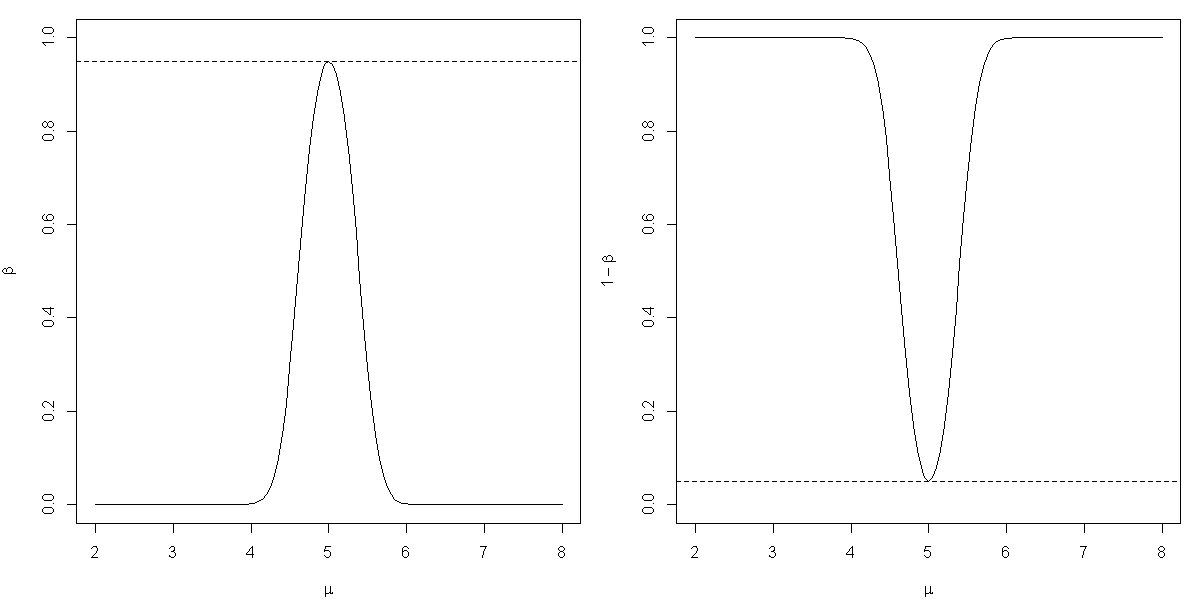
\includegraphics[height=.6\textheight]{img/power.png}
    \caption{Probabilidad de error tipo II $\beta(\mu)$ y función de potencia $\pi(\mu)=1-\beta(\mu)$ para el test que plantea en la hipótesis nula $H_0:\mu_{0}=5$.}
    \label{fig:potencia-2}
  \end{figure}
\end{frame}



\begin{frame}{\color{rosee}Ejemplo 2}\small
  
    Consideremos la hip\'otesis nula de que el peso medio de estudiantes
    hombres de cierta universidad es 68 kilogramos, contra la
    alternativa de que es diferente. Determine la región de rechazo y calcule el $p$-valor si observa $\overline{x}_{\text{obs}}= 69.68$.
    \begin{description}
    \item[$H_0$:] $\mu = 68$
    \item[$H_1$:] $\mu \neq 68$
    \end{description}
    Supongamos $\alpha = 0.05$, $\sigma = 3.6$ y $n=36$. Luego,
    \begin{align*}
      \mathcal R
      &=  \left\{\overline{X}_{36}\leq 68 - 1.96\cdot3.6/\sqrt{36}\right\} \cup
        \left\{\overline{X}_{36}\geq 68 + 1.96\cdot3.6/\sqrt{36}\right\} \\
      &= \left\{\overline{X}_{36}\leq 66.8 \right\} \cup
        \left\{\overline{X}_{36}\geq 69.2\right\}.
    \end{align*}
  

    \begin{align*}
      \text{$p$-valor}
      &= P(| \overline{X}_{36}- 68| \geq | \overline{x}_{\text{obs}} -68| \text{ cuando $H_0$ es verdadera} ) \\
      &= P(| \overline{X}_{36}- 68| \geq 1.68 \text{ cuando $H_0$ es verdadera})\\
      &= 2P(\overline{X}_{36}\geq 69.68 \text{ cuando $H_0$ es verdadera}) \\
      &= 0.005.
    \end{align*}
    ¿Cómo concluye el test? Como $\overline{x}_{\text{obs}}\in \mathcal{R}$ se rechaza $H_0$ con un nivel $\alpha=0.05$.

\end{frame}


\begin{frame}{\color{rosee}Test cola izq. para $\mu$ si $X_i\stackrel{iid}{\sim}N(\mu,\sigma^2)$ y $\sigma^2$ es conocida}\small
 Queremos testear
    \[H_0: \mu \geq \mu_0 \quad\text{vs}\quad H_1:\mu < \mu_0\]
  
Consideremos el siguiente estadístico estadístico: $t(\munderbar{X})=\frac{\sqrt{n}(\overline{X}_n-\mu)}{\sigma}$
    ¿Qu\'e distribuci\'on tiene el estad\'istico bajo $H_0$?
      \begin{equation*}
        Z = \dfrac{\sqrt{n}(\overline{X}_n- \mu_0)}{\sigma} \sim N(0,1)
      \end{equation*}

  Proponemos un test de la forma
  \[\text{rechazo} \; H_0 \Leftrightarrow \overline{X}_n \leq k\]
  con $k$ que verifica 
  \[\alpha = \max_{\mu \geq \mu_0} P_{\mu}(\text{rechazar} \; H_0) =
  \max_{\mu \geq \mu_0} P_{\mu}(\overline{X}_n \leq k)\]
 Entonces rechazamos $H_0$ si $Z \leq z_{1-\alpha} $, es decir si
      \[\overline{X}_n\leq \mu_0 - z_{1-\alpha}\frac{\sigma}{\sqrt{n}}.\]
    
\end{frame}

\begin{frame}{\color{rosee}Ejemplo 3}\small
  % Devore Example 9.2
    El tiempo de secado de un tipo de pintura bajo condiciones
    espec\'ificas se distribuye normalmente con media 75 min y desv\'io
    est\'andar 9 min. Se toma una muestra de tamaño $n=25$ y considere $\alpha = 0.01$.
    
\medskip
 Se dise\~nó un aditivo qu\'imico para disminuir el tiempo
    de secado. Se cree que el tiempo de secado con este aditivo
    tambi\'en se distribuye de manera normal con $\sigma=9$.   Sea $\mu$ el tiempo de secado medio cuando el aditivo es
    usado. 

    \medskip
    
    Las hip\'otesis son \[H_0: \mu = 75\text{ vs }H_1: \mu < 75\]
    
    \medskip
    
Rechazamos $H_0$ si $Z < -z_{0.99}=2.326$ o
    equivalentemente si
    \[\mathcal{R} = \left \{\overline{X}_{25}\leq 70.8 \right\}\]

    Observemos que $\alpha$ se calcula usando la distribuci\'on bajo
    $H_0$ mientras que para el c\'alculo de $\beta$ necesitamos conocer
    la distribuci\'on del estad\'istico del test para los valores de $\mu$ bajo $H_1$. Calcule $\beta(72)$, $\beta(70)$ y $\beta(67)$. ¿Qué puede concluir?

 \end{frame}

 \begin{frame}{\color{rosee}Ejemplo 3 (continuación)}
    \begin{align*}
      \beta(72)
      &= P_{\mu=72}(\mbox{error de tipo II}) \\
      &= P_{\mu=72}(\mbox{no rechazar }H_0) \\
      &= P_{\mu=72}(\overline{X}_{25}> 70.8) = 0.7486
    \end{align*}
Porque, cuando $\mu=72$, $\overline{X}_{25}\sim N(72;9/\sqrt{25}))$.
    \begin{align*}
      \beta(70) &= 1- \Phi\left(\frac{70.8-70}{1.8}\right) = 0.33\\
      \beta(67) &= 1- \Phi\left(\frac{70.8-67}{1.8}\right) = 0.0174
    \end{align*}
    Sin embargo, la probabilidad de un error de tipo II es grande cuando
    $\mu = 72$ (un peque\~no alejamiento de $H_0$), un poco menor cuando
    $\mu = 70$ y bastante menor cuando $\mu = 67$. %(un desv\'io sustancial respecto de $H_0$).

 
\end{frame}


 \begin{frame}{\color{rosee}Ejemplo 3 (continuación)}\small
  \begin{exampleblock}{Ejemplo (pintura)}
    \begin{figure}
      \centering
      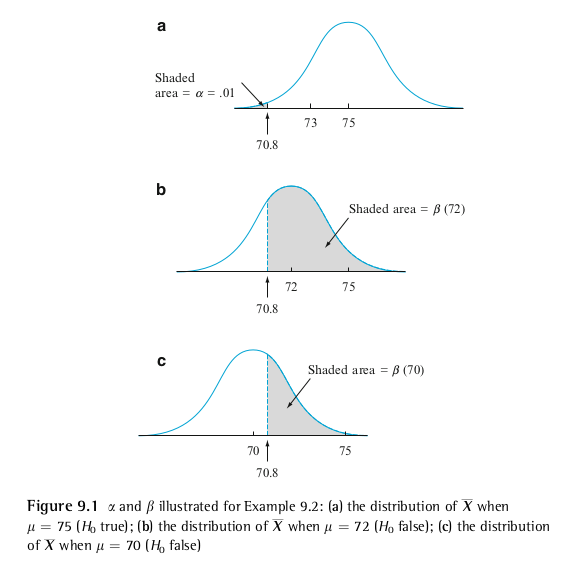
\includegraphics[height=.8\textheight]{img/pintura-devore.png}
    \end{figure}
  \end{exampleblock}
\end{frame}

 \begin{frame}{\color{rosee}Ejemplo 3 (continuación)}
      Si hubi\'eramos considerado la hip\'otesis nula
    \[H_0: \mu \geq 75\] tenemos un valor de $\alpha$ para cada valor de
    $\mu \geq 75$:
    \[\alpha(75), \quad \alpha(75.8), \quad\alpha(76.5), \quad \dots\]
    Es f\'acil ver que $\alpha(75)$ es el mayor de los errores de tipo
    I.

 En general el peor escenario ocurre en el borde. \textbf{Por lo tanto, si bien bajo $H_0$ el parámetro $\mu$ puede tomar muchos valores, acotamos la probabilidad de error de tipo I por ``el peor caso posible''. Es decir, tomamos el valor de $\mu$ bajo $H_0$ de manera que, dado el valor crítico $c$ a partir del cual se rechaza $H_0$, la distribución de $t(\munderbar{X})$ bajo $H_0$ tiene el mayor error de tipo $I$. En este caso, dicho valor es $\mu=75$.}
\end{frame}

\begin{frame}{\color{rosee}Test cola der. para $\mu$ si $X_i\stackrel{iid}{\sim}N(\mu,\sigma^2)$ y $\sigma^2$ es conocida}\small
 Queremos testear
    \[H_0: \mu \leq \mu_0 \quad\text{vs}\quad H_1:\mu > \mu_0\]
  
  Proponemos un test de la forma, con estadístico: $t(\munderbar{X})=\frac{\sqrt{n}(\overline{X}_n-\mu)}{\sigma}$
    ¿Qu\'e distribuci\'on tiene el estad\'istico bajo $H_0$?
      \begin{equation*}
        Z = \dfrac{\sqrt{n}(\overline{X}_n- \mu_0)}{\sigma} \sim N(0,1)
      \end{equation*}

  Proponemos un test de la forma
  \[\text{rechazo} \; H_0 \Leftrightarrow \overline{X}_n \geq k\]
  con $k$ que verifica 
  \[\alpha = \max_{\mu \leq \mu_0} P_{\mu}(\text{rechazar} \; H_0) =
  \max_{\mu \leq \mu_0} P_{\mu}(\overline{X}_n \geq k)\]
 Entonces rechazamos $H_0$ si $Z \geq z_{1-\alpha} $, es decir si
      \[\overline{X}_n\geq \mu_0 + z_{1-\alpha}\frac{\sigma}{\sqrt{n}}.\]
    
\end{frame}


\begin{frame}{\color{rosee}Test cola der. para $\mu$ si $X_i\stackrel{iid}{\sim}N(\mu,\sigma^2)$ y $\sigma^2$ es conocida}\small
  Buscamos $k$
  $$P_{\mu}(\overline{X}_n \geq k) = P \left ( \frac{\sqrt{n}(\overline{X}_n
      -\mu)}{\sigma} \geq \frac{\sqrt{n}(k -\mu)}{\sigma}\right)
  = \underbrace{1- \Phi \left (\frac{\sqrt{n}(k -\mu)}{\sigma}
    \right)}_{\text{funci\'on creciente en } \mu}$$
  Entonces el valor de $\mu$ que comete con mayor probabilidad el error de tipo I es cuando $\mu=\mu_0$
  $$\alpha = \max_{\mu \leq \mu_0}
  1-\Phi\left(\frac{\sqrt{n}(k-\mu)}{\sigma}\right) = 1-\Phi
  \left ( \frac{\sqrt{n}(k-\mu_0)}{\sigma}\right)$$
  Despejamos $k$
  $$k = \mu_0 + z_{1-\alpha} \frac{\sigma}{\sqrt{n}}$$
  Entonces el test rechaza $H_0$ cuando 
  $$\frac{\sqrt{n}(\overline{X}_n- \mu_0)}{\sigma} \geq z_{1-\alpha}$$
\end{frame}

\begin{frame}{\color{rosee}Test cola der. para $\mu$ si $X_i\stackrel{iid}{\sim}N(\mu,\sigma^2)$ y $\sigma^2$ es conocida}\small
  Calculemos la funci\'on de potencia del test
  \begin{align*}
    \pi(\mu) 
    &= P_{\mu} \left( \overline{X}_n \geq \mu_0 + z_{1-\alpha}
      \frac{\sigma}{\sqrt{n}} \right)\\ 
    &=  P_{\mu} \left( \frac{\sqrt{n}(\overline{X}_n -
      \mu)}{\sigma} \geq \frac{\sqrt{n}(\mu_0-\mu)}{\sigma} +
      z_{1-\alpha} \right)\\
    &= 1 -
      \Phi\left(\frac{\sqrt{n}(\mu_0-\mu)}{\sigma} + z_{1-\alpha} \right)
  \end{align*}
  Entonces
  $$ \pi(\mu) = 1-
  \Phi\left(\frac{\sqrt{n}(\mu_0-\mu)}{\sigma} + z_{1-\alpha} \right)$$

    Observemos que 
  \begin{itemize}
  \item Si aumenta $\alpha$ aumenta la potencia 
  \item Si aumenta $\mu$ aumenta la potencia
  \item Si aumenta $n$ aumenta la potencia
  \item Si se reduce $\sigma$ aumenta la potencia
  \end{itemize}
\end{frame}



\begin{frame}{\color{rosee}Test cola der. para $\mu$ si $X_i\stackrel{iid}{\sim}N(\mu,\sigma^2)$ y $\sigma^2$ es conocida}\small

Gráfico de la función de potencia para valores de $\mu$ cuando, bajo $H_0$, $\mu_0=0$.
  \begin{figure}
    \centering
    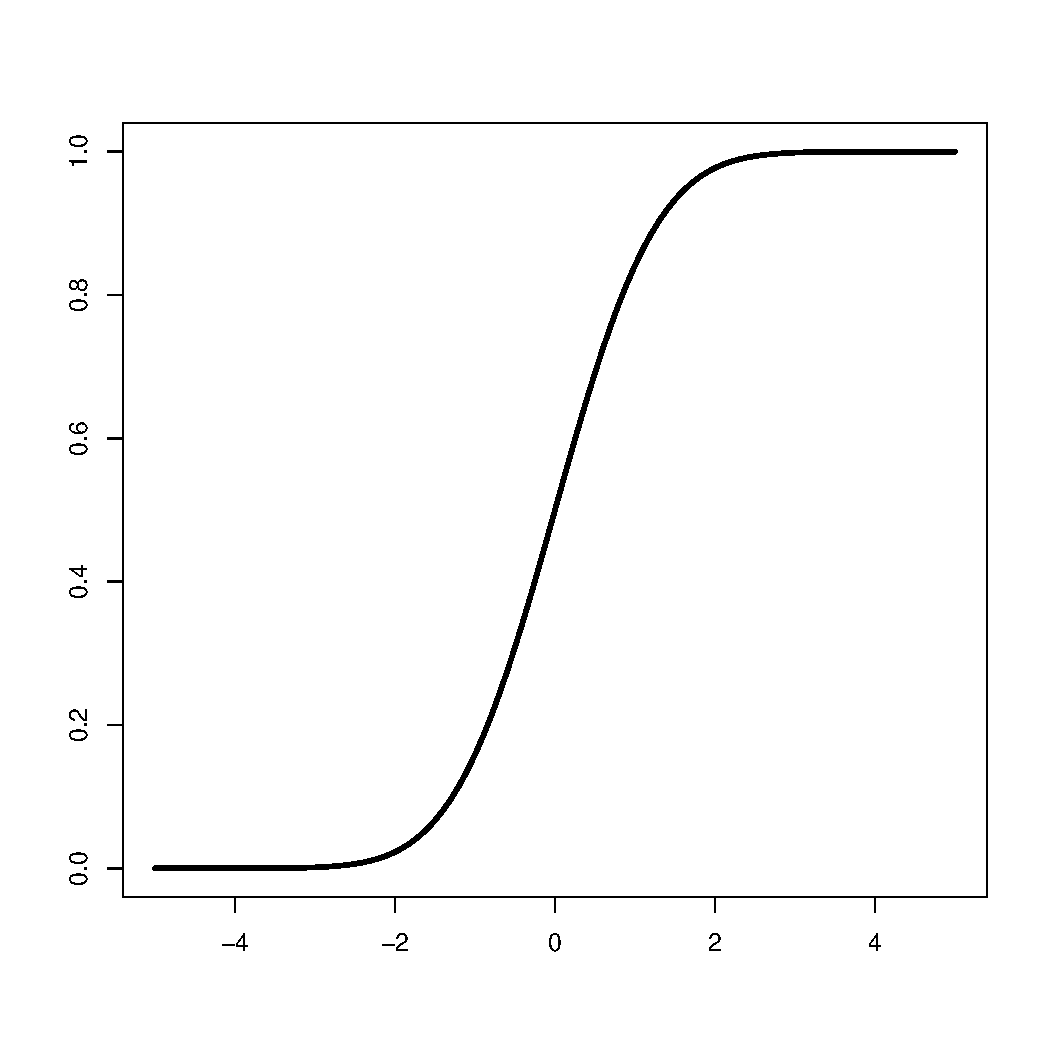
\includegraphics[height=.7\textheight]{img/potencia-1.pdf}
    \caption{Funci\'on de potencia $\pi(\mu)$.}
    \label{fig:potencia-1}
  \end{figure}
\end{frame}



\begin{frame}{\color{rosee}Fijado $\alpha$, busquemos $n$ de manera que $\beta$ sea ``pequeño''}\small
  ¿Cu\'anto deber\'ia ser el tama\~no de muestra para lograr una buena
  potencia del test para $\alpha$ fijo y una alternativa espec\'ifica
  fija?
  
  \bigskip
  Supongamos que queremos testear:
  \begin{description}
  \item[$H_0$:] $\mu = \mu_0$
  \item[$H_1$:] $\mu > \mu_0$
  \end{description}
  con un nivel de significaci\'on $\alpha$ cuando conocemos $\sigma$.
\end{frame}

\begin{frame}{\color{rosee}Fijado $\alpha$, busquemos $n$ de manera que $\beta$ sea ``pequeño''}\small
Para el test $H_0:\mu=\mu_0$ vs $H_1:\mu>\mu_0$ consideremos una hipótesits alternativa espec\'ifica $\mu = \mu_0 + \delta$, 
  \begin{figure}
    \centering
    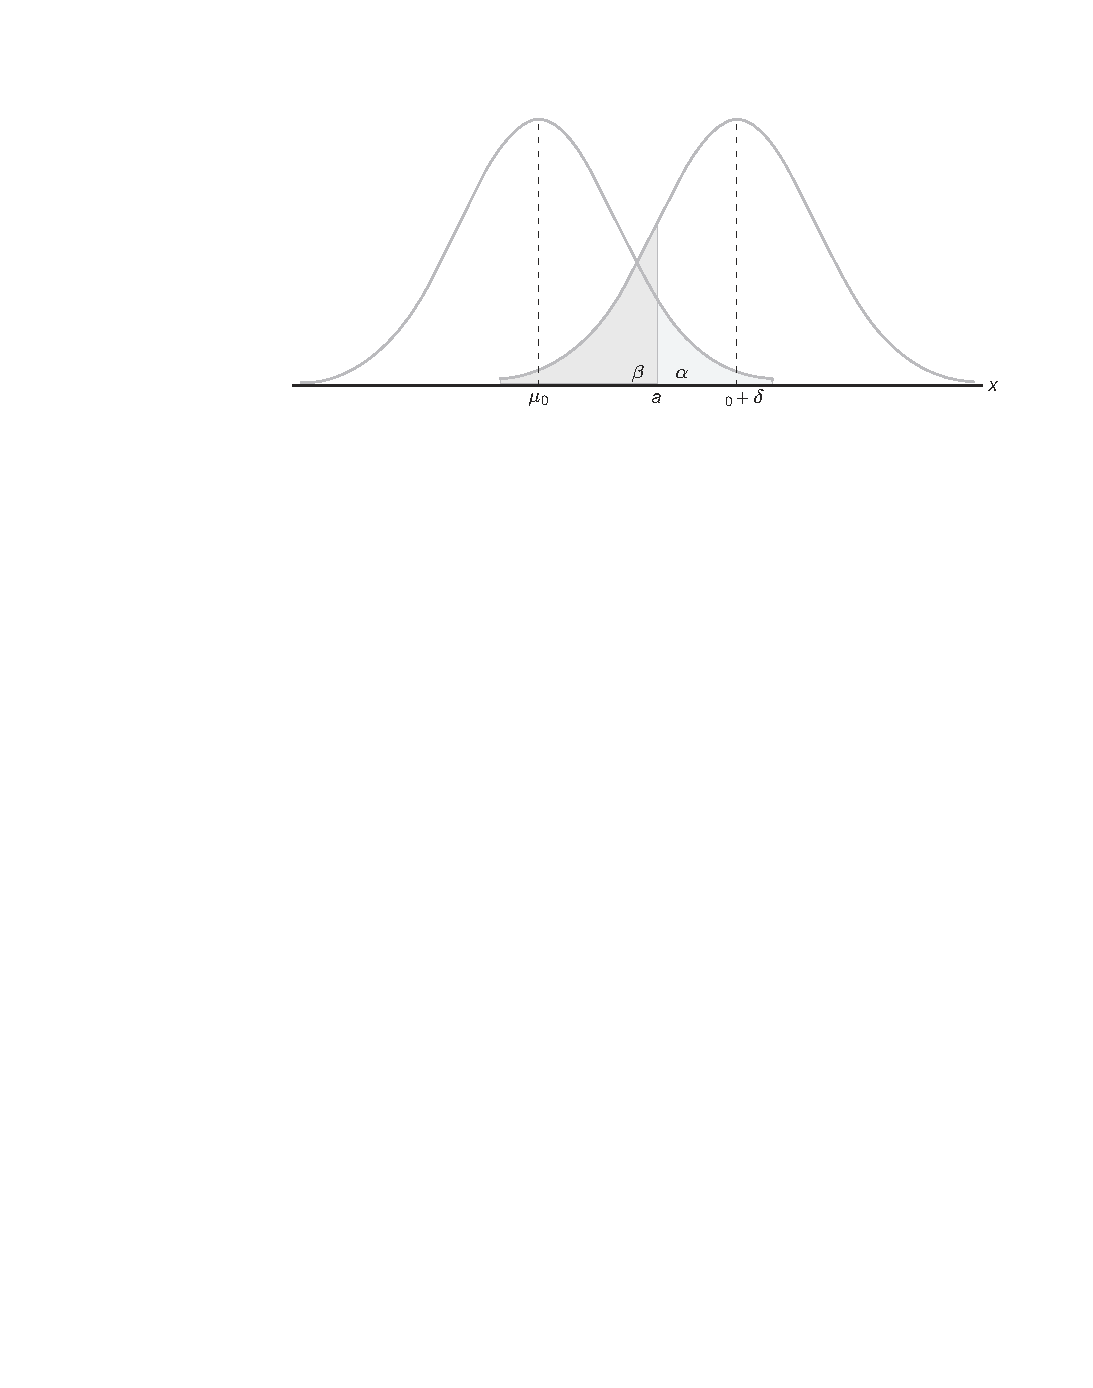
\includegraphics[height=.4\textheight]{img/eleccion_n.pdf}
  \end{figure}
  la potencia del test es 
  \[ \pi(\mu_{0}+\delta)  = P_{\mu = \mu_0 + \delta} \left(\overline{X}_n\geq \mu_0 +
      z_{1-\alpha}\frac{\sigma}{\sqrt{n}} \right) = P_{\mu = \mu_0 + \delta} (Z \geq -
      \delta \sqrt{n}/\sigma + z_ {1-\alpha})\]
\end{frame}

\begin{frame}{\color{rosee}Fijado $\alpha$, busquemos $n$ de manera que $\beta$ sea ``pequeño''}\small

Para el test $H_0:\mu=\mu_0$ vs $H_1:\mu>\mu_0$
  \begin{itemize}
  \item Habiendo fijado una probabilidad de erorr de tipo I, $\alpha$, ¿de qu\'e tama\~no deber\'ia ser la muestra $n$ para que nuestro
    test tenga una potencia $1-\beta$?
    \[ 1-\beta  = \pi(\mu_{0}+\delta) = P_{\mu = \mu_0 + \delta}\left(Z \geq - \delta \frac{\sqrt{n}}{\sigma} +
      z_{1-\alpha}\right)\] Entonces,
      $$
      \beta(\mu_0 + \delta) = P_{\mu = \mu_0 + \delta}\left(Z \leq - \delta \frac{\sqrt{n}}{\sigma} +
      z_{1-\alpha}\right)
      $$
      y por lo tanto
    \[-\delta \frac{\sqrt{n}}{\sigma} + z_ {1-\alpha} = z_{1-\beta} \Rightarrow
      \textcolor{blue}{n = \frac{(z_{1-\beta}+z_ {1-\alpha})^2
          \sigma^2}{\delta^2}}\]

  \end{itemize}
 \end{frame}


\begin{frame}{\color{rosee}Resumen test exacto si $X_i\stackrel{iid}{\sim} N(\mu,\sigma^2)$ y $\sigma^2$ es conocida}
\begin{itemize}
\item Para testear en cada uno de los casos: \medskip
	\begin{center}
		$H_{0}$: $\mu \geq \mu _{0} \qquad \qquad \qquad H_{0}$: $\mu =\mu _{0}\qquad \qquad \qquad
		H_{0}$: $\mu \leq \mu _{0}$
		
		$H_{1}$: $\mu <\mu _{0} \qquad \qquad \qquad H_{1}$: $\mu \neq \mu _{0}\qquad \qquad \qquad
		H_{1}$: $\mu >\mu_{0}$
	\end{center}
	\medskip
\item Utilizamos el estadístico de contraste	$\overline{X}_n\sim N\left(\mu,\frac{\sigma^2}{n}\right)$.  \medskip
%\begin{itemize}
\item Fijamos la signficatividad $\alpha$ y definimos las regiones de \underline{rechazo} $\mathcal{R}$:\medskip
%\end{itemize}
\end{itemize}


\scalebox{0.8}{
$ \left\{\overline{X}_n: \overline{X}_n\leq \mu_0 - z_{1-\alpha}\frac{\sigma}{\sqrt{n}}\right\} \quad \left\{\overline{X}_n: |\overline{X}_n-\mu_0| \geq z_{1-\alpha/2}\frac{\sigma}{\sqrt{n}}\right\} \quad \left\{\overline{X}_n: \overline{X}_n\geq \mu_0 +  z_{1-\alpha}\frac{\sigma_0}{\sqrt{n}}\right\} $}


\begin{itemize}
\item Garantizamos en los 3 casos que: $ \displaystyle\max_{\mu \in H_0}P_{H_0}\left(\overline{X}_n\in \mathcal{R}\right) \leq \alpha.$\medskip
\end{itemize}
\end{frame}

\begin{frame}
%	\frametitle{Región de rechazo del test}
\smallskip
Las regiones de rechazo se pueden escribir en términos de $Z = \frac{\overline{X}_n- \mu_0}{\sigma_0/\sqrt{n}}$:
	\begin{figure}
		\centering
		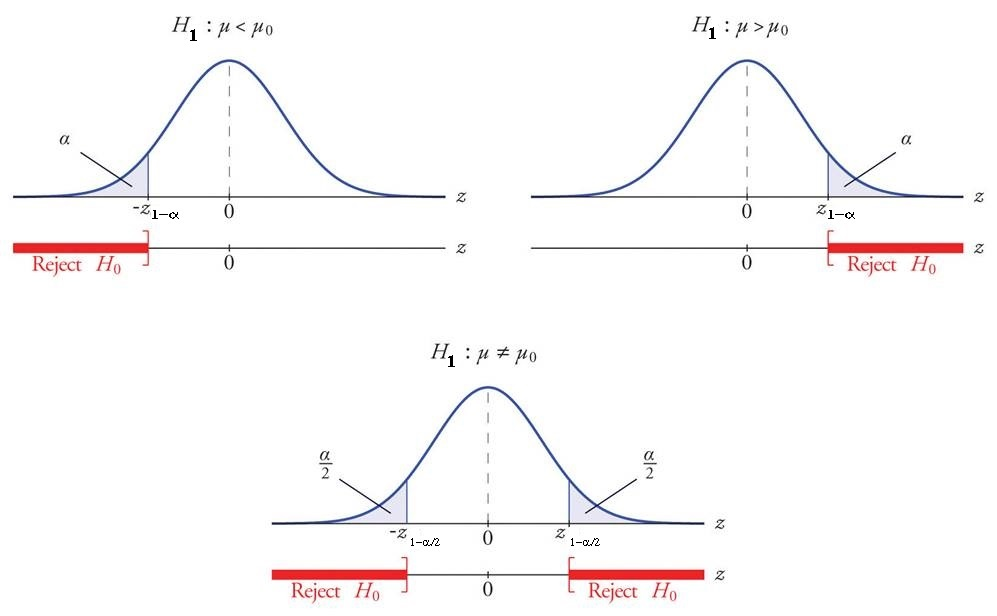
\includegraphics[width=0.75\linewidth]{img/regionmedia.jpg}\\
	\end{figure}
\begin{center}
    \scalebox{1}{
$ \left\{Z: \frac{\overline{X}_n- \mu_0}{\sigma_0/\sqrt{n}} \leq -z_{1-\alpha}\right\} \quad \left\{Z: \left|\frac{\overline{X}_n- \mu_0}{\sigma_0/\sqrt{n}}\right| \geq z_{1-\alpha/2}\right\} \quad \left\{Z: \frac{\overline{X}_n- \mu_0}{\sigma_0/\sqrt{n}}\geq z_{1-\alpha}\right\}$}
\end{center}
\end{frame}

\begin{frame}{\color{rosee}Resumen TH para $\mu$ si $X_i\stackrel{iid}{\sim} N(\mu,\sigma^2)$}
    \begin{center}
        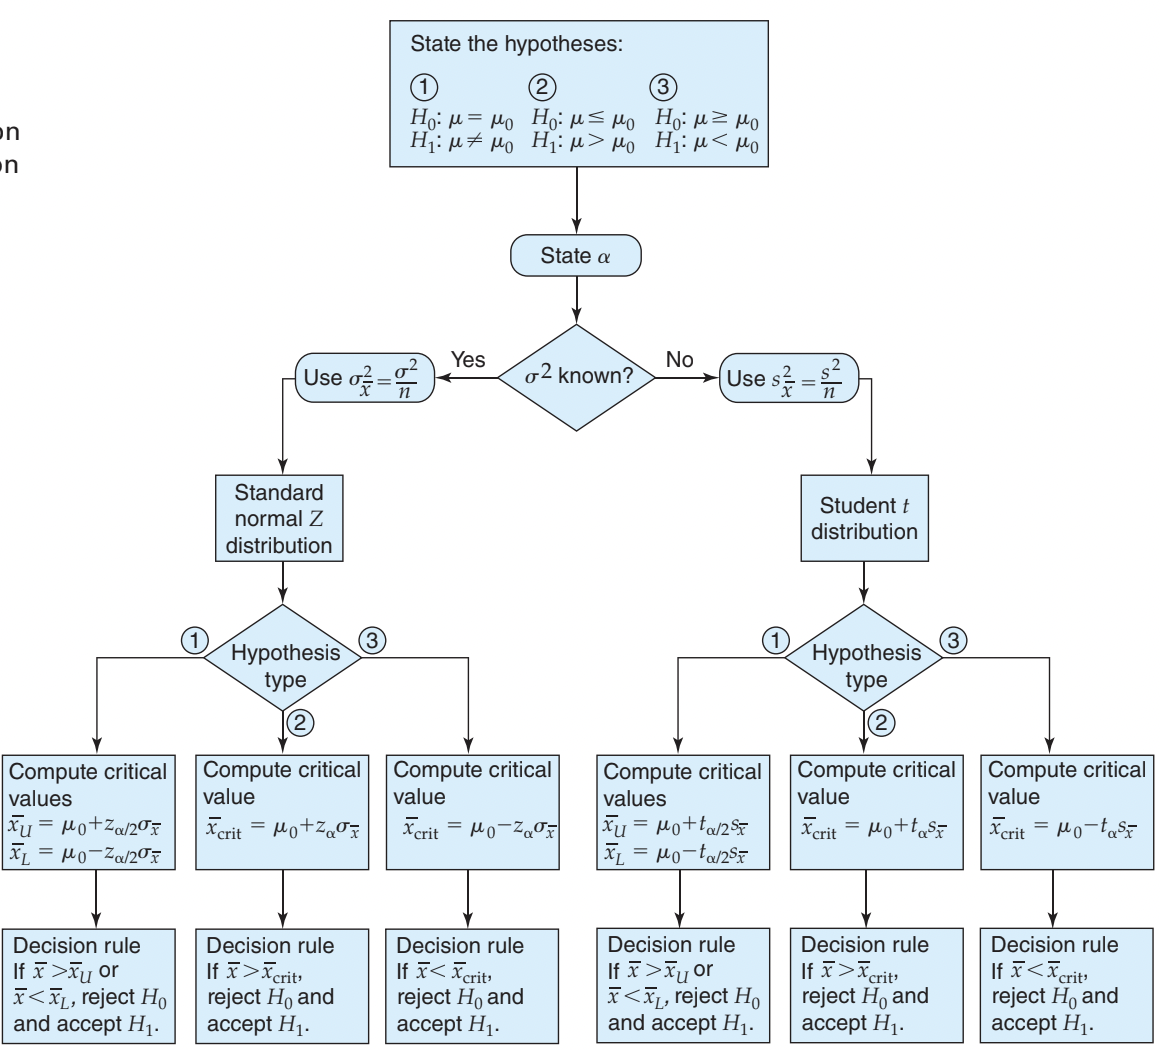
\includegraphics[scale=0.4]{slides6/img/testnormal.png}
    \end{center}
\end{frame}

\begin{frame}{\color{rosee}Dualidad entre los test y los intervalos}\small
\begin{itemize}
\item Consideremos el test:
\[
\begin{cases}
H_{0}: \mu =\mu _{0}\\
H_{1}: \mu \neq \mu _{0}
\end{cases}
\]
\item Para una significatividad $\alpha$ fija, la región de rechazo \textbf{serán los valores de }$\overline{X}_n$ que cumplan que:
$$\mathcal{R} = \left\{\overline{X}_n:|\overline{X}_n-\mu_0| \geq z_{1-\alpha/2}\frac{\sigma}{\sqrt{n}} \right\} $$
\item Por lo tanto la región de \underline{no rechazo} $\mathcal{R}^C$ se puede escribir como:
$$\mathcal{R}^C= \left\{\overline{X}_n:\overline{X}_n -z_{1-\alpha/2}\frac{\sigma}{\sqrt{n}}\leq \mu_0 \leq \overline{X}_n +z_{1 -\alpha/2}\frac{\sigma}{\sqrt{n}} \right\} $$
\item \textbf{Corolario}: Para un test de significatividad $\alpha$, si  $\mu_0$ cae \medskip
\begin{itemize}
\item Dentro del intervalo de confianza $1-\alpha \Rightarrow$ no rechazamos $H_0$.\medskip
\item Fuera del intervalo de confianza $1-\alpha \Rightarrow$ rechazamos $H_0$.
\end{itemize}
\end{itemize}
\end{frame}

\begin{frame}{\color{rosee}Test para $\mu$ si $X_i\stackrel{iid}{\sim}N(\mu,\sigma^2)$, $\sigma^2$ desconocida}
\begin{itemize}
\item Para cualquiera de los siguientes conjuntos de hipótesis:
	\begin{center}
		$H_{0}$: $\mu \geq \mu _{0}\qquad \qquad H_{0}$: $\mu = \mu _{0}\qquad \qquad	H_{0}$: $\mu \leq \mu _{0}$
		
		$H_{1}$: $\mu < \mu _{0}\qquad \qquad H_{1}$: $\mu \neq \mu _{0}\qquad \qquad
		H_{1}$: $\mu >\mu _{0}$
	\end{center}

	
\item El estadístico de contraste es:
	$$T=\frac{\overline{X}_n-\mu _{0}}{S /\sqrt{n}}\sim t_{n-1}$$

\item Una vez elegimos $\alpha$, las regiones de rechazo serán:	

\begin{center}
\scalebox{0.85}{
$\hspace{-3em} \left\{\overline{X}_n: \overline{X}_n\leq \mu_0 - t_{1-\alpha}\frac{S}{\sqrt{n}}\right\} \quad \left\{\overline{X}_n: |\overline{X}_n-\mu_0| \geq t_{1-\alpha/2}\frac{S}{\sqrt{n}}\right\} \quad \left\{\overline{X}_n: \overline{X}_n\geq \mu_0 +  t_{1-\alpha}\frac{S}{\sqrt{n}}\right\} $}
\end{center}
	
%\item \textbf{Test exacto} (vale para $n$ pequeño).
\end{itemize}
\end{frame}


\begin{frame}{\color{rosee}Ejemplo de test $t$}
\small
Durante el mes pasado, en las farmacias de la capital el precio de un medicamento seguía una distribución normal de media \$1780. Este mes, en una muestra de 16 farmacias, se estimó que $\overline{X}_{16}=\$1900$ y $s=\$250$. ¿Aumentó el precio medio del medicamento?
%		\pause
\begin{enumerate}
\item En primer lugar planteamos el test:
\[
\begin{cases}
		H_{0}: \mu \leq \mu_0=1780\\
		H_{1}:\mu >\mu_0=1780
\end{cases}
\]
\item Elige $\alpha$ (el tamaño del test) y determina la región crítica.\medskip
$$ \alpha= 0.05 \text{ y } t_{15,1-\alpha }=1.753\Rightarrow R_\alpha = \Big\{ T = \frac{\overline{X}-\mu _{0}}{S/\sqrt{n}} > 1.753 \Big\}$$

\item Con los datos de la muestra $T=\frac{1900-1780}{250/\sqrt{16}}=1.92$.\medskip
\item Rechazamos $H_0$ con $\alpha = 0.05$, hay evidencia de aumento precio medio.
\end{enumerate}			
\end{frame}


\begin{frame}{\color{rosee}Sobre el cálculo del $p$-valor (resumen) }\small

El \textbf{$p$-valor} se puede pensar como el menor valor de significación $\alpha$ con el cual la \textbf{hipótesis nula puede ser rechazada} \underline{dados los datos de la muestra} bajo $H_0$.

\medskip
\begin{itemize}
\item Si $H_0:\mu \leq \mu_0$ y el estadístico de contraste vale $T=t_0$: $$p-\text{valor} = P_{H_0}\big( T \geq t_0\big).$$
\item Si $H_0:\mu \geq \mu_0$ y el estadístico de contraste vale $T=t_0$: $$p-\text{valor} = P_{H_0}\big( T \leq t_0\big).$$
\item Si $H_0:\mu = \mu_0$ y el estadístico de contraste vale $T=t_0$: $$p-\text{valor} = 2 \min\left\{P_{H_0} (T \leq t_0),P_{H_0}( T \geq t_0)\right\}.$$

\end{itemize}
En todos los casos rechazamos $H_0$ si el $p$-valor cumple que $p-\text{valor}<\alpha$.
\end{frame}

\end{document}